%\addcontentsline{toc}{subsection}{Note on the available R package : \texttt{evdbayes}}
\section{Methods }\label{sec:meth}


There exists a bunch of methods to make Bayesian inference, including different algorithms but also different implementations of these algorithms, i.e. different packages, programming interfaces or languages. We have vastly looked for methods that are the most suited for our nonstationary GEV analysis, which was not an easy task.

The pioneering and reference Bayesian R package in EVT is \texttt{evdbayes} from \citet{ribatet_users_2006}. Launched more than years ago, it is still the only available package on CRAN to do Bayesian inference in EVT with MCMC techniques. We have passed a long time trying to understand and make relevant analysis through this framework. However, we had problems to "open black-box" and truly understand its structure. For example, it was not possible to tune correctly the algorithm in order to reach the target posterior distribution for a nonstationary model. Moreover, \citet{hartmann_bayesian_2016} states that \texttt{evdbayes} only implements the Metropolis-Hastings (MH) (Algorithm \ref{algo:mh} in \hyperref[app:mh]{Appendix \textbf{\ref{app:mh}}}).
Hence, we decided to develop our own methods in the developed R package. We decided to implemented not only the MH,  but also the Gibbs sampler (Algorithm \ref{algo:gib} in \hyperref[app:mh]{Appendix \textbf{\ref{app:mh}}}).
 We give a brief summary of the methods we have used (or only considered) for this chapter : 
 
 \begin{itemize}
 	\item[$\blacktriangleright$] The \texttt{evdbayes} package discussed above. Although the documentation is complete, the methods are rather not intuitive nor very flexible. Moreover, we can feel the evolution of the R language this last decade.
 	
 	\item[$\blacktriangleright$] From \emph{our functions} in the R package, where we implemented both the MH algorithm and the Gibbs sampler. This allowed us to have a thorough understanding of these algorithms. We also used it to carefully tune the hyperparameters and obtain relevant and reliable results, that we could visually plot in the best manner.
 	
 	\item[$\blacktriangleright$] From \emph{HMC algorithm} using \emph{STAN language}, which is the most efficient but also the most complex to use. While offering state-of-the-art methods for both execution and diagnostic of the generated Markov chains, it also presents much theoretical technicalities, but also practical. This explains the limited amount of results we have been able to produce with this outstanding method.
 	 	
 	 \item[$\vartriangleright$] The \emph{Ratio of Uniform} method from the \texttt{\textbf{r}evdbayes} package (see \citet{northrop_2017_revd}), which internally makes use of the \texttt{rust} package to simulate a random sample from the required posterior distribution,  is an other acceptance-rejection type of simulation algorithm.
   Even if this method is different from the traditional MCMC, the package also makes use of a low-level language (C++) to perform the most time-consuming tasks. Hence, in terms of efficiency, this method is worth studying for Bayesian inference with extreme values.   
 \end{itemize}
 Using a compiled language either in preference to R or as a subroutine called from R typically results in a two-fold or three-fold
 speed increase over optimized R code for iterative simulation algorithms such as in MCMC simulation, see e.g. \citet{stan_development_team_stan_2012}.

Regarding the prior $\pi(\theta)$, the different methods discussed in \hyperref[sec:prior]{Section \textbf{\ref{sec:prior}}} are available in the \texttt{evdbayes} framework. Since we will mostly rely on our functions and we have no experts' advices, we will rather use vague priors as in \hyperref[sec:noninfoprior]{Section \textbf{\ref{sec:noninfoprior}}}, and hence not implement all these priors in our package. 

Since learning a new language (STAN) for such a complex task was very limiting, we will only present the results that we obtained for the selected nonstationary model (\hyperref[sec:baycomp]{Section \textbf{\ref{sec:baycomp}}}) with the functions we have constructed. However, we now briefly present the results obtained with the three methods for the stationary model. 


\section{Stationary GEV Model : Algorithms' Comparison}\label{sec:baystatio}


This section presents the results obtained for the stationary GEV model in order to compare the different methods discussed above and in \hyperref[sec:baymcmc]{Section \textbf{\ref{sec:baymcmc}}}. 

We note that for this particular model, the results are very similar to those obtained with the \texttt{evdbayes} framework and are not shown here. We empirically verified that this package uses the MH algorithm, even if we think that  \texttt{evdbayes} can use the Gibbs sampler, unlike \citet[pp.6]{hartmann_bayesian_2016} stated in their article.

Since this is not possible to evaluate analytically the complete posterior in (\ref{bayeseq}) for this model, we will use MCMC approximations. The same non-informative (near-flat) normal priors will be used
in the three methods.

\subsection{Comparison of the Methods}


Figure \ref{fig:mhgibhmc} in \hyperref[app:bayfig]{Appendix \textbf{\ref{app:bayfig}}}
shows the parameters' chains generated for each parameters by the different algorithms. 
We clearly see the chains updating one at a time in the MH algorithm while the updates are individual in the Gibbs sampler and in the HMC, implying traceplots that have the same shape for each parameters with the MH algorithm. This is related to the acceptance rates, where we can clearly visualize their effects : they are increasing from the left to the right plots, i.e. from chains that have a succession of constant episodes (left plots) to chains that resemble to those of a white noise process.
This clearly impacts the efficiency of the underlying algorithm since the parameter space of the target distribution will be more quickly visited when the acceptance rate(s) is (are) high, depending also on the structure and on other parameters of the algorithm. 


\begin{table}[!htbp] \centering 
	\caption{Comparison of three Bayesian MCMC algorithms with $N= 2000$ samples with a Burn-in period $B=500$ with the frequentist MLE for the stationary model. Parameters are estimated by their posterior mean, effective sample sizes $(N_{\text{\emph{eff}}})$ (\ref{eq:neff}) for estimating the mean are displayed for Bayesians, and standard errors for frequentist. } 
	\label{tab:mhgib} 
	\begin{tabular}{@{\extracolsep{5pt}} ccccc} 
		\toprule
		& \textbf{MH} $(N_{\text{eff}})$  & \textbf{Gibbs} $(N_{\text{eff}})$  & \textbf{HMC} $(N_{\text{eff}})$  & \textbf{MLE} (s.e.) \\ 
		\midrule
		Location $\mu$  & $30.596\ (183)$ & $30.567\ (232)$  & $30.5978\ (\boldsymbol{769})$& $30.587\ (0.216)$ \\ 
		Scale $\sigma$ & $2.101 \ (183)$ & $2.117\ (145)$ & $2.100\ (\boldsymbol{621})$ & $2.081\ (0.155)$ \\ 
		Shape $\xi$ & $-0.2445\ (183)$ & $-0.2449\ (144)$ & $-0.2433 \ (\boldsymbol{541})$  & $-0.254\ (0.067)$ \\ 
		\midrule[0.005mm]   		  
		Computation time &  $0.39$ sec. &  $2.23$ sec. & $0.72$ sec.  &  \\
		\bottomrule
	\end{tabular} 
\end{table} 

We can see from Table \ref{tab:mhgib} that all the estimates are very close to each other and vary in a very low order of magnitude. Even if all the Bayesian methods are giving satisfying results, it is important to discover which method is the most efficient. 


 \subsubsection*{Metropolis-Hastings and Gibbs Sampler}


Regarding the choice of the proposals, we took multivariate (MH) and univariate (Gibbs) Normal distributions since symmetric distributions have better properties and are more easily handled.
We tuned the standard deviations of the proposals by a \emph{trial-and-error} approach. Even with an univariate proposal (Gibbs), it is difficult task to tune each standard deviations separately to achieve desirable acceptance probabilities for all parameters.

The MH algorithm is the best in terms of computation time since it only requires one update within each iterations, and hence only one log-posterior computation (the most computationally time consuming task in the algorithms). As the Gibbs sampler evaluates an update for each parameters separately, it takes more time to execute. This can be seen on Algorithms \ref{algo:mh} and \ref{algo:gib}, where the latter involves a nested loop. 

Since the autocorrelations in the chains is the same for the MH algorithm, the number of effective samples will be the same for each parameters, while it will highlight the convergence issues with Gibbs sampling, and we see that the shape parameter have more difficulty to attain the target posterior stationary distribution than $\mu$.

However, other technicalities have to be taken into account when choosing between these algorithms,  and even these two "accept-reject" methods have lots of similarities, we will rather use Gibbs sampling since it is more conveniently producing a sequence of low dimension simulations that still converge to the right target. This will quite more easily handled when considering nonstationary models with increasing number of parameters (\hyperref[sec:baycomp]{Section \textbf{\ref{sec:baycomp}}}).

 \subsubsection*{Hamiltonian Monte-Carlo}

As discussed in \hyperref[sec:hmc]{Section \textbf{\ref{sec:hmc}}}, the efficiency of the HMC algorithm can directly be visualized with Table \ref{tab:mhgib}. Indeed, the model executes in only $0.82$ seconds since the log-posterior evaluation is handled into a lower-level of abstraction, and yields a drastically higher number of effective samples $(N_{\text{eff}})$. We can visualize it at the following \href{https://proto4426.shinyapps.io/ShinyStanGEV_converged/}{URL}\footnote{\url{https://proto4426.shinyapps.io/ShinyStanGEV_converged/}} that the chains are very poorly autocorrelated. This is a Shiny application provided by the package \texttt{rstan} together with \texttt{shinystan} that allow to locally deploy this kind of visualization from an executed model in a few lines of code only, see \textbf{/Scripts-R/}\texttt{Shiny\_stan\_test.R} on the \href{https://github.com/proto4426/PissoortThesis/}{repository}. 

This tool were particularly useful in our case since we have ran this algorithm a very high number of times and it was extremely difficult to attain convergence. 
An impressive number of diagnostics, often difficult to understand but well documented inside the application, helped us to resolve the convergence issues. In fact, this problem is linked to the property of the GEV distribution. Since the support depends on the parameter values, i.e. $x_*=\mu-\sigma\cdot\xi^{-1}$ and $_*x=-\infty$ as we are under an EV-Weibull model, we must be clever with the declarations of the parameters. Otherwise, zero or undefined density values could be picked as valid parameter values by STAN. The difficulty was also probably related to \hyperref[likgevintro]{Section \textbf{\ref{likgevintro}}} where we have shown that with a parameter $\xi$ being relatively near the problematic region, the likelihood computations could cause convergence problems in the STAN program. 


 In addition of being a lower-level language, the STAN language has several benefits : 
 
 \begin{itemize}
 	\item  Although the HMC algorithm is rather complex to implement, the STAN community offers its help and proposes lots of interesting tools that helps for the modeling, such as the automatically generated Shiny applications shown above. These applications provide an outstanding amount of information. The \texttt{bayesplot} also provides a bunch of outstanding visualizations from an executed STAN model. Moreover, a very active 		 \href{https://groups.google.com/forum/#!forum/stan-users}{STAN community} driven by the founders of STAN will be happy to assist with your problems. 
 	
 	\item It allows for more flexibility through the direct mathematical formulation of the desired model, and the probabilistic computations that will result in the STAN program. Moreover, a large library
 	of distributions is available.
 	
 	\item While the program structure is more straightforward and user-friendly for this kind of problems, every STAN programs can be called in R, and we can then benefit from all the tools and packages that R proposes.
 \end{itemize}
However, the major drawback is that it is a new language to learn with new methods to learn, with all the problems and errors associated. Together with the convergence issues discussed above, we were unfortunately not able to compute the nonstationary models with this method and we keep going with the Gibbs sampler.


\section{Nonstationary GEV : Model Comparisons}\label{sec:baycomp}

Although information criteria such as the BIC informed us in \hyperref[sec:anagev]{Chapter \textbf{\ref{sec:anagev}}} that the nonstationary model with a linear trend on the location parameter is the best suited among all the parametric models for the location and the scale parameters, we decided to adopt the similar sequential methodology, starting with the simplest model (Gumbel) to more complex parametric models and by using the Bayesian techniques from \hyperref[sec:modcompbay]{Section \textbf{\ref{sec:modcompbay}}} to compare models. Thence, we will be able to compare the results between the frequentist and the Bayesian frameworks, and perhaps could reinforce our confidence that the model selected in \hyperref[sec:anagev]{Chapter \textbf{\ref{sec:anagev}}} is the best suited.
We could be based on the frequentist's analysis of the previous chapters to select some (subset of) more relevant models to analyze, but we decided to take the same models in order to facilitate the comparisons. Besides that, the number of parametric models that we can propose  is limited.


The Gibbs sampler will then be used for each models. To limit the influence of the four randomly selected starting values, we take a burn-in period of length $B=N/2$. Taking $N_\text{tot}=4\cdot 1000$ for each parameter's chains, this leaves us with $N=2000$ samples.
With tools from \hyperref[sec:convbay]{Section \textbf{\ref{sec:convbay}}}, we diagnosed the convergence of each chains separately for each models.

\subsubsection*{Bayes Factor}

The Bayes Factor is the most straightforward statistic in the Bayesian paradigm when one wants to compare models.
Unfortunately, we did not find any ways to compute the marginal likelihood (\ref{eq:marglik}) which is an intractable $2$ to $6$-dimensional integral for the models considered. It is necessary and often a big issue when computing the Bayes factor in practice. 
We were absolutely not able to compute for our models even with the efficient method proposed by \citet{chib_1995}.

 \subsubsection*{Predictive Information Criteria}
 
 
 Another way that allows to compare model is by using the predictive information criteria discussed in \hyperref[sec:predacur]{Section \textbf{\ref{sec:predacur}}}. Rather than evaluating the quality of fit of a model in terms of its accuracy with the observed data, these criteria evaluate the predictive accuracy,
 which is to a certain extent, relatively similar. 
  
 
 For each of the four generated chains with dispersed starting values, we evaluate separately the predictive information criteria  to check that variability of the criteria is reassuringly very small between chains. The discrepancies between the chains are very small for most models, which is a good sign. Surprisingly, we observed much more variability in the criteria for simpler models. We obtained the following standard deviations for the most simple and the most complex models :
 \begin{equation*}
 \begin{aligned}
\sigma(\text{DIC}|\text{Gumbel}) = 157, \qquad \sigma(\text{WAIC}|\text{Gumbel}) = 78, \\ 
\sigma(\text{DIC}|\text{Cubic}) = 5, \qquad \qquad 
\sigma(\text{WAIC}|\text{Cubic}) = 3 \quad
\end{aligned} 
 \end{equation*}
The complete results are displayed in Table \ref{tab:comp_mod_bay}, computed by the mean of the criteria for each parameter chain with a different starting value. 

\begin{table}[!htbp] 
	\centering \caption{Comparisons of nested GEV models with nonstationary parameters computed by Gibbs sampler for $N=2000$ by means of predictive accuracy criteria.} 
	\vspace{-.1cm}
	\label{tab:comp_mod_bay} 
	\begin{tabular}{@{\extracolsep{5pt}} ccccc} 
		\toprule
		\textbf{Model} & DIC & WAIC  & Computation Time (sec.) \\
		\midrule
		stationary Gumbel & $517.4$  & $515.6$ &  $0.98$ \\
		stationary GEV  & $576.6$ & $540.1$  &   $1.9$ \\
		\textbf{linear in} \boldsymbol{$\mu(t)$} & $\boldsymbol{720.9}$ & $\boldsymbol{602.5}$&   $3.9$ \\
		quadratic in $\mu(t)$ & $484.6$ & $483.9$ &  $4.9$ \\
		linear in $\mu(t)$ and $\sigma(t)$ & $486.6$ & $485.1$  & $5.4$ \\
		cubic in $\mu(t)$ & $450.3$ & $487.8$  & $7.8$ \\
		\bottomrule
	\end{tabular}
	\vspace{-.15cm}
\end{table} 
The model that is the most predictive accurate is the nonstationary GEV model with a linear trend on the location, as previously chosen with other criteria. We notice that the difference with the other models is very large. The more complex models considered have a very low amount of predictive accuracy, probably because they overfit the data and they do not capture the signal.
 Since we were not able to compare models with the Bayes factor, one could argue that using carefully Bayesian model averaging could improve the results. We discuss this issue at the \hyperref[sec:bmaxp]{end of this Chapter}, but averaging with the more complex models should not be beneficial at first sight.
 The computation time is obviously higher for models that have more parameters since each parameters requires one update (see Algorithm \ref{algo:gib}).
 
  

\section{Nonstationary GEV with Linear Model on Location}\label{sec:bay_nonsta}


From the above Bayesian model selection with predictive criteria, but also the more straightforward selection made during \hyperref[sec:anagev]{Chapter \textbf{\ref{sec:anagev}}} (see e.g. Tables \ref{tab:comp_mod0} and \ref{tab:comp_mod}) in a frequentist setting, we decide to go through with this parsimonious nonstationary model, and see how a Bayesian analysis can help with inferences.

We write our model for the annual maxima $X_t$ as  
\begin{equation*}
X_{t}\sim \text{GEV}\big(\mu(t), \sigma, \xi\big), \qquad \text{with} \ \ \mu(t)= \mu_0+\mu_1\cdot t,
\end{equation*}
where $t=[1901,2016]$ but in practice, we will take the rescaled values of $t$ by $t^{*} = \frac{t - \bar{t} }{|t|}$ that yield better properties of the  Gibbs sampler. 
We have then four parameters $\theta=(\mu_0,\mu_1,\nu,\xi)$, where $\nu=\log\sigma$. We take independent vague prior distributions for each parameters :
\begin{equation*}
\pi(\mu_0)\sim\mathcal{N}(30,40^2),\quad \pi(\mu_1)\sim\mathcal{N}(0,40^2),\quad \pi(\nu)\sim\mathcal{N}(0,10^2),\quad
\pi(\xi)\sim\mathcal{N}(0,10^2).
\end{equation*}
Values are recommended by \citet[chap.13]{dey_extreme_2016}. We verified that relatively small changes in the hyperparameters do not significantly influence the results.
For numerical reasons, will compute the unnormalized posterior on the log scale, i.e.

\begin{equation}\label{eq:logpost}
\log\pi(\theta|\boldsymbol{x})\propto \log\pi(\theta)\cdot \ell(\theta|\boldsymbol{x}),
\end{equation}
in order to facilitate the numerical computations while not affecting the results.


\subsubsection*{MCMC Algorithm : Gibbs Sampler}

Since this is not possible to evaluate analytically (\ref{bayeseq}) for this model, we will use the MCMC method to approximate the true target posterior distribution. 

We will use the Gibbs sampler (Algorithm \ref{algo:gib}) as it is the most effective, especially in a nonstationary setting, i.e. when the number of parameters to evaluate is high. As the computation time is not a real issue for our application, this sampler is the perfect perfect candidate.



\subsubsection*{Starting Values}

\hyperref[sec:anagev]{Chapter \textbf{\ref{sec:anagev}}} numerically optimized the log-likelihood to compute the MLE in the frequentist setting. Now, we will use the same technique but on the log-posterior (\ref{eq:logpost}).
To control the influence of the starting values, we run $c=4$ chains, each having different starting values. This $[4\times 4]$ matrix $\boldsymbol{\theta_0}$ of starting values are randomly selected from a multivariate normal distribution that is over-dispersed relative to the target. To make this clear, we write the little Algorithm \ref{algo:start}.

\vspace{.3cm}
\begin{algorithm}[H]
	\SetAlgoLined
	\begin{enumerate}
		\item Take the optimized values from log-posterior from (\ref{eq:logpost}), say $\hat{\theta}$.
		\item \textbf{For} $i=1,\ldots,c$ \quad \textbf{do}
		\begin{itemize}
			\item Sample the $i$-th starting value $\theta_{0,i}$ from
			\begin{equation*} 
      \theta_{0,i}\sim \mathcal{N}_4\Big(\hat{\theta}, \ k\times \Sigma^l\Big)
			\end{equation*}
			where $\Sigma^l$ is the estimated covariance matrix of the log-posterior optimized values $\hat{\theta}$.
		\end{itemize}
	\end{enumerate}
	\caption{Compute $c$ starting values $\boldsymbol{\theta_0}$}\label{algo:start}
\end{algorithm}
\vspace{.3cm}
Note that $\hat{\theta}$ can simply be the MLE if the priors are near-uniform. To obtain over-dispersed values, $k$ must be high. We take $k=50$ in our application to increase our confidence that the whole parameter space has been visited. This value can be easily tuned to obtain more desirable starting values. We display the obtained starting values in Table \ref{tab:startbay}.
\begin{table}[!htbp] \centering 
	\caption{Starting values taken for the Gibbs sampler, from Algorithm \ref{algo:start} with $k=50$. } 
	\label{tab:startbay} 
	\begin{tabular}{@{\extracolsep{5pt}} c|cccc} 
\toprule
    %& \multicolumn{4}{c}{Parameters} \\
		& $\mu_0$ & $\mu_1$ & $\log\sigma$ & $\xi$ \\ 
\midrule
		$\theta_{0,1}$ & $30.193$ & $5.730$ & $0.960$ & $-0.349$ \\ 
		$\theta_{0,2}$& $31.849$ & $4.402$ & $0.447$ & $0.257$ \\ 
	$\theta_{0,3}$ & $31.487$ & $0.478$ & $1.156$ & $-0.529$ \\ 
	$\theta_{0,4}$ & $31.636$ & $-0.011$ & $-0.024$ & $0.130$ \\ 
\bottomrule
	\end{tabular} 
\end{table} 
We see the great dispersion in the starting values. The shape parameter includes both positive and very negative values, while the trend parameter $\mu_1$ includes negative values but also (very) high values.
The generated chains will be displayed in Figure \ref{fig:mixchains}.


\subsubsection*{Proposal Distribution}


The implemented Gibbs sampler (Algorithm \ref{algo:gib}, or \texttt{gibbs.trend.own} in our R package) has univariate normal distributions as proposal distributions. This choice could be debatable but we will take it for its convenience since it is symmetric, and results would not really change as long as the acceptance rates are acceptable and the algorithm converges : it would only impact the algorithm's efficiency. Hence for each parameter $j=1,\ldots,4$, we have at iteration $t$ of the algorithm

\begin{equation}
p_{t,j}\Big(\theta^{(j)}_*|\theta^{(j)}_{t-1}\Big) \sim \mathcal{N}\Big(\theta^{(j)}_{t-1},\big(\sigma^{(j)}_p\big)^2 \Big),
\end{equation}
where $\boldsymbol{\sigma_p}=(0.5, 1.9, 0.15,0.12)'$ is the $4$-dimensionnal vector containing the proposal's standard deviations of each parameter. This vector is a hyperparameter that we have tuned by trial-and-error to obtain the recommended acceptance rates for each parameter's chains : all between $36\%$ and $43\%$ for the $4\cdot 4=16$ computed chains. If generalization is required, it is easily possible to find an automatic way to achieve this instead of relying on trial-and-error. 


\subsubsection*{Computations} 

It took only $3.5$ seconds for $N_{\text{tot}}=4\cdot 1000$ iterations. For each of the $4$ chains that have different starting values, we took a burn-in period of $500$, and we are thus left with $N=(4000-4\cdot 500)=2000$ iterations. It should probably be better to take more iterations as it is quite fast, but for better visualizations, we will keep $N=2000$.
Note that running the different chains in parallel is straightforward and should decrease the computation time by a factor of $\approx 2$, but it is not necessary here for such a small $N_{\text{tot}}$.
 
 
\subsection{Diagnostics}

Before any inference on the generated chains, it is vital to check whether the samples reached their target stationary distribution or not.
We remind that no diagnostics can prove convergence, but their combined use will increase our confidence that it indeed happened.
This section will sometimes rely on the \texttt{coda} package for some diagnostics. These diagnostics are described in \hyperref[app:convdiag]{Appendix \textbf{\ref{app:convdiag}}}

 Figure \ref{fig:mixchains} shows the traceplots of the chains after burn-in. Even if the convergence seems to occur quite fast from the complete traceplots of the chains, we preferred removing $50\%$ to increase our confidence that the starting values have no influence.
\begin{figure}
	\centering
	\begin{subfigure}[b]{0.99\textwidth}
		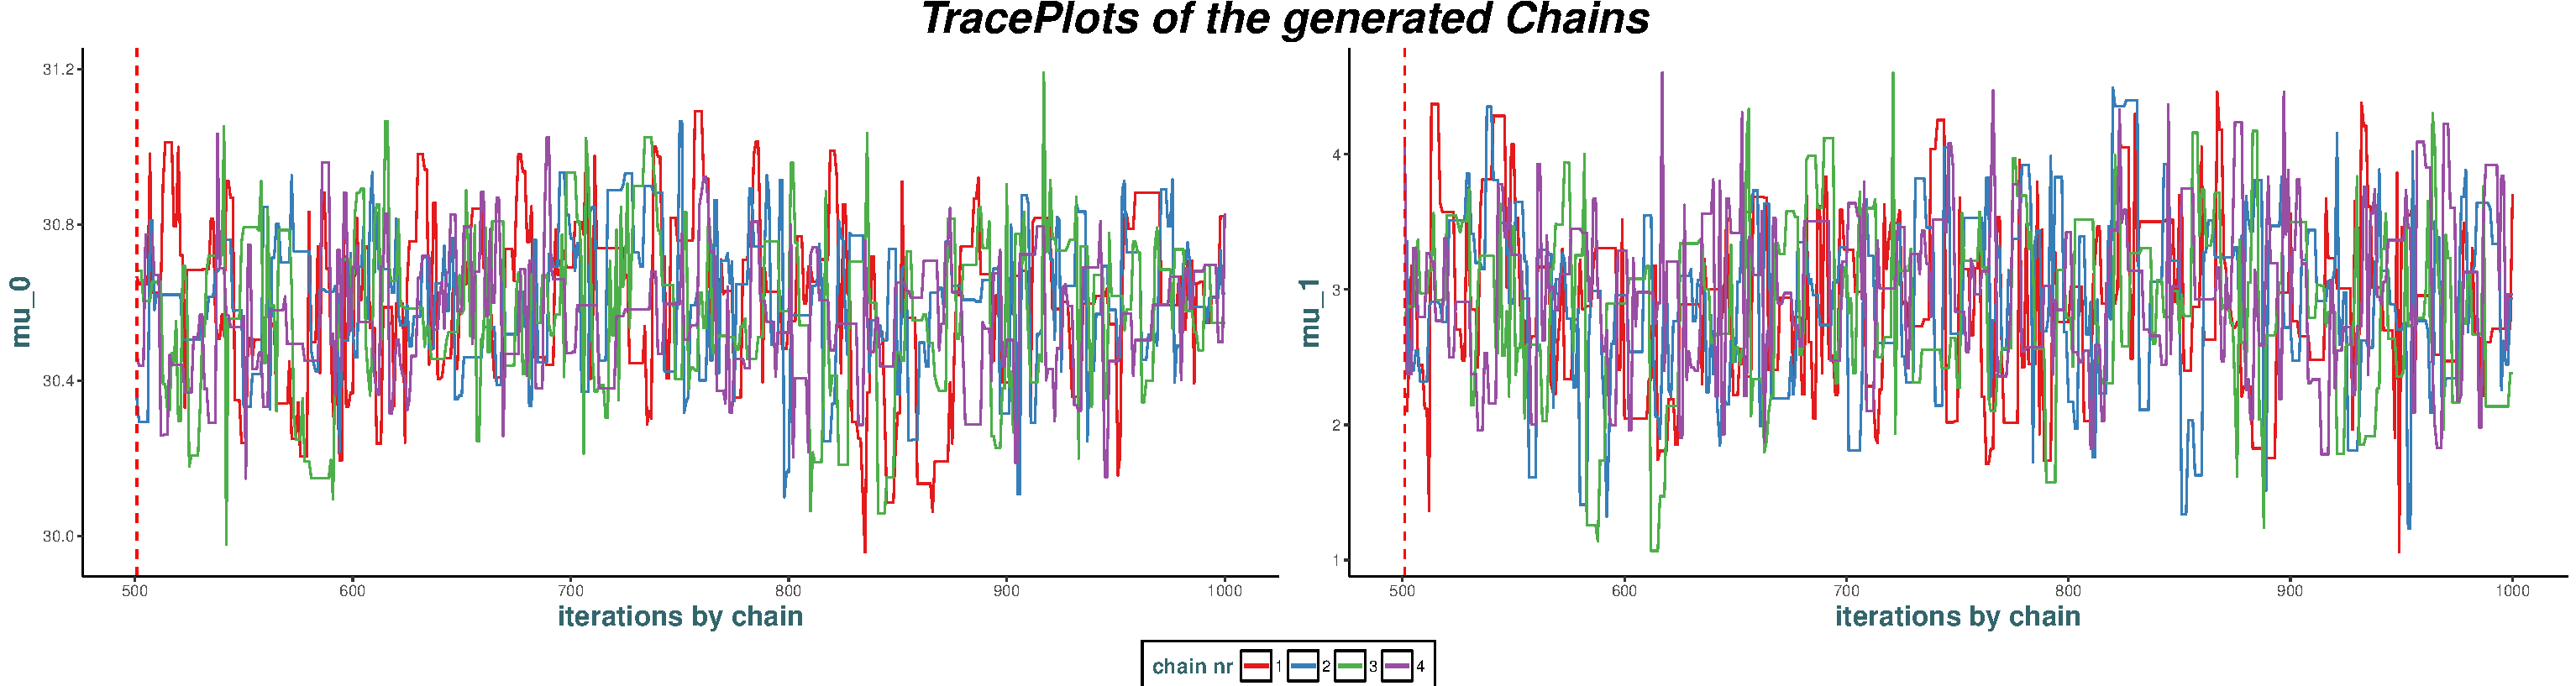
\includegraphics[width=1\linewidth]{chains1.pdf}
	\end{subfigure}
	
	\begin{subfigure}[b]{0.99\textwidth}
		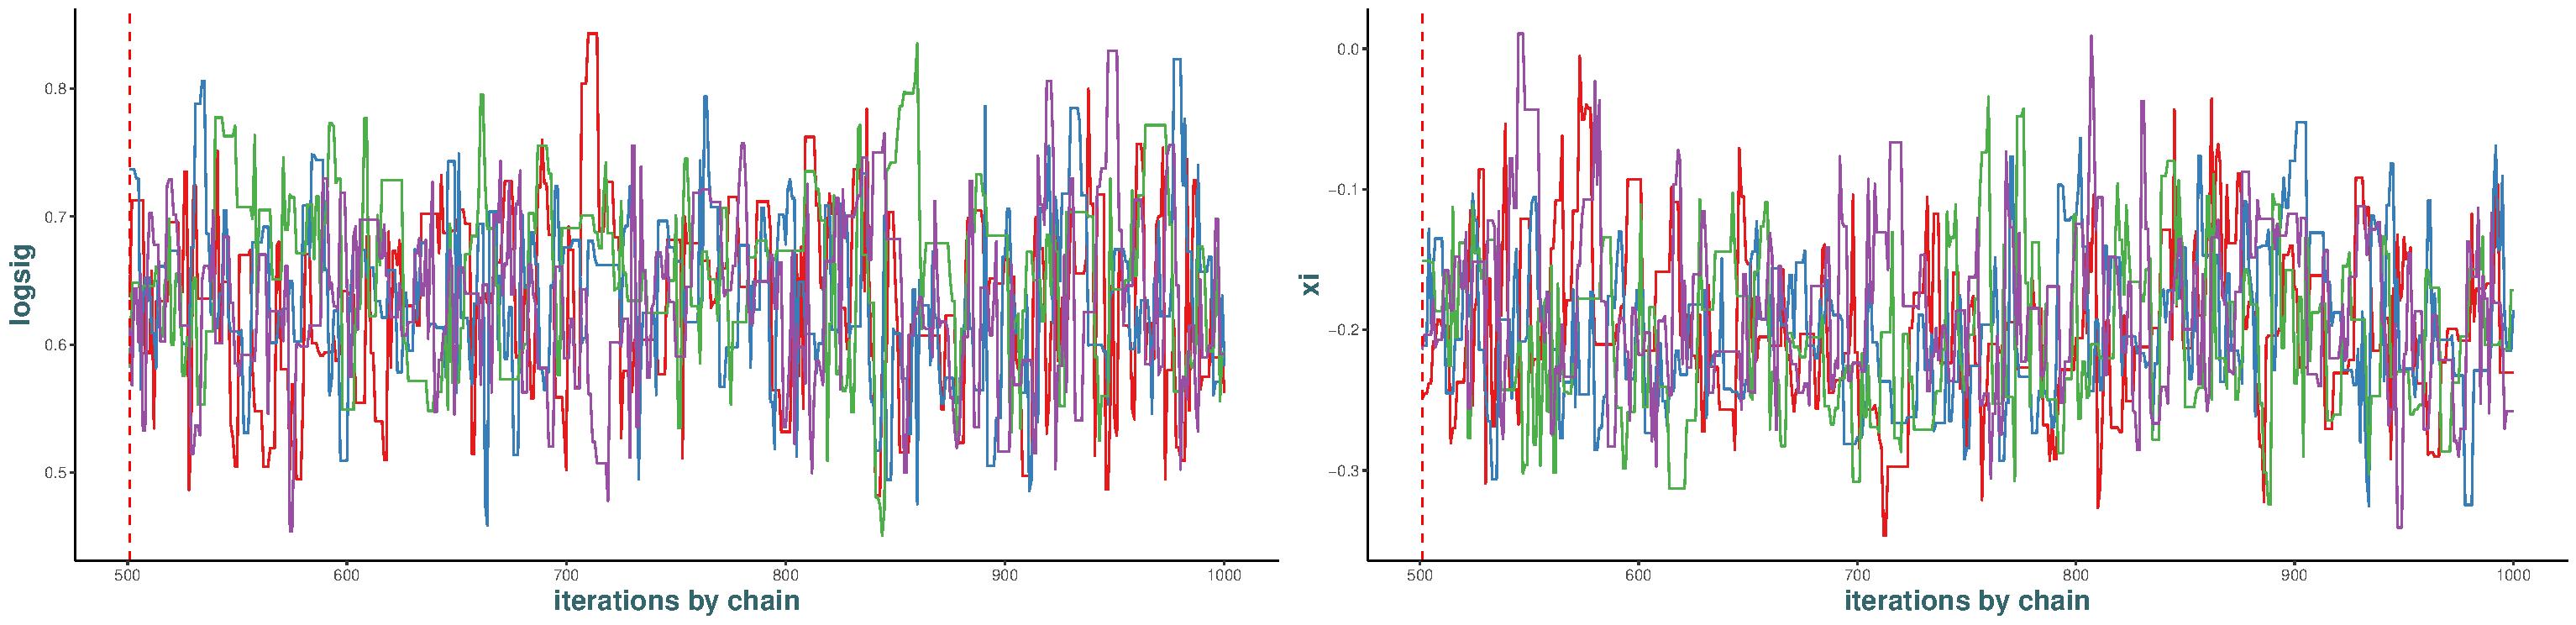
\includegraphics[width=1\linewidth]{chains2.pdf}
	\end{subfigure}
	\caption{Traceplots of the chains with $4$ different starting values obtained with our Gibbs sampler for the nonstationary model with linear model on location. Note that the location parameter of the trend $\mu_1$ is of different order as before because we are based on the rescaled values $t^*$ of $t$. We will transform it back  later for inferences (Table \ref{tab:postq}). }\label{fig:mixchains}
\end{figure}
Each parameter show chains that are mixing very well, reinforcing our confidence that the over-dispersed starting values we used have no influence on the target stationary distribution. 
Thense, we now gather all the chains with different starting values into a single chain, to obtain one single chain of size $N=2000$ for each parameter.


\subsubsection*{Gelman-Rubin}

The Gelman-Rubin diagnostic compares the behavior of the randomly initialized chains. It computes the $\hat{R}$ (\ref{eq:rhat}) or \emph{shrink factor} which measures the mixing of the chains. If convergence occurred, the $\hat{R}$ will be $1$.
The corresponding results are displayed in Figure \ref{fig:gelmdiag} in \hyperref[app:bayfig]{Appendix \textbf{\ref{app:bayfig}}}. It clearly shows that the parameter $\mu_0$ attains very quickly the values that indicate convergence, and somewhat surprisingly, it is yet faster for $\mu_1$.
As expected, it is a bit more tedious for the shape parameter, but it is especially slow for $\log\sigma$ for which it takes at least $500$ iterations before $\hat{R}<1.1$. However, since all parameters have $\hat{R}$ going very close to $1$ at the end of the series, the number $N=2000$ of iterations should be sufficient.



\subsubsection*{Correlations within and between chains}


\begin{itemize}
	\item The \textbf{autocorrelations} of each parameter's Markov chain depicted in Figure \ref{fig:autocor} in \hyperref[app:bayfig]{Appendix \textbf{\ref{app:bayfig}}} are quickly decreasing with the lag. Again, it seems more problematic for $\log\sigma$ and $\xi$ as the decrease is slower, showing more dependence inside their respective chain.	
	We have computed the effective sample size $N_{\text{eff}}$ from (\ref{eq:neff}), i.e. the sample size after correction for the autocorrelation in the chains :
	\begin{equation}
		N_{\text{eff}}^{(\mu_0)} = 389, \qquad 	N_{\text{eff}}^{(\mu_1)} = 436, \qquad 	N_{\text{eff}}^{(\nu)} = 194, \qquad	N_{\text{eff}}^{(\xi)} = 217.
	\end{equation}
	We can see the link of these values with the autocorrelations in Figure \ref{fig:autocor}. All these very high are not very high.
	
	\item The \textbf{cross-correlation} between the parameters' Markov chains are depicted in Figure \ref{fig:crosscorr} in \hyperref[app:bayfig]{Appendix \textbf{\ref{app:bayfig}}}. We have compared these values with the Fisher information matrix that we transformed in a correlation matrix, and we have found very similar values except for the correlation between the location parameters $\mu_0$ and $\mu_1$ (probably because of the rescaling of $t$).
\end{itemize}


\subsubsection*{Geweke}

This diagnostic tests the equality of the first $10\%$ of a chain with the mean computed from the second half of the chain. The chain has been partitioned in order to repeat the test $20$ times.
Figure \ref{fig:geweke} in \hyperref[app:bayfig]{Appendix \textbf{\ref{app:bayfig}}} shows the results. Quite surprisingly, $\mu_0$ has $6$ rejected values out of $20$, but these are really at the limit. Shape and log scale parameters are still somewhat problematic. However, we notice that this diagnostic is very diffuse, in the sense that results will be very different from one test to another with different generated chains with the same method.


\subsubsection*{Raftery and Lewis and Thinning}

One last diagnostic comes from \citet{raftery1992} and provides interesting values on the chains. These are shown in Table \ref{tab:raf} in \hyperref[app:bayfig]{Appendix \textbf{\ref{app:bayfig}}}.
Relatively high autocorrelations in the chains are again highlighted here. The advised values for $N$ are slightly higher to those used, and the Burn-in period advised is very low.  



\subsubsection*{Conclusion}

From all the above results, i.e. especially the relatively high correlations within and between chains, it is recommended to increase the number of iterations $N$. Since the computational time is not real concern, it would be easy to increase $N$. But in order to keep the same chains as presented above, and to keep the analysis homogeneous, we just decrease the burn-in period by $50\%$. We are now left with $N=3000$ samples for each chains. 


\subsection{Inference}\label{sec:bayinfci}

Now that we have shown confidence that the Gibbs sampler has converged, the Markov chains are supposed to have been from their target posterior stationary distribution. It is nos possible to make reliable inferences on the GEV parameters with these samples.

We first present the results in Figure \ref{fig:postdens} with the corresponding Markov chains' Kernel posterior densities for each parameters.
\begin{figure}[!htb]
	\centering	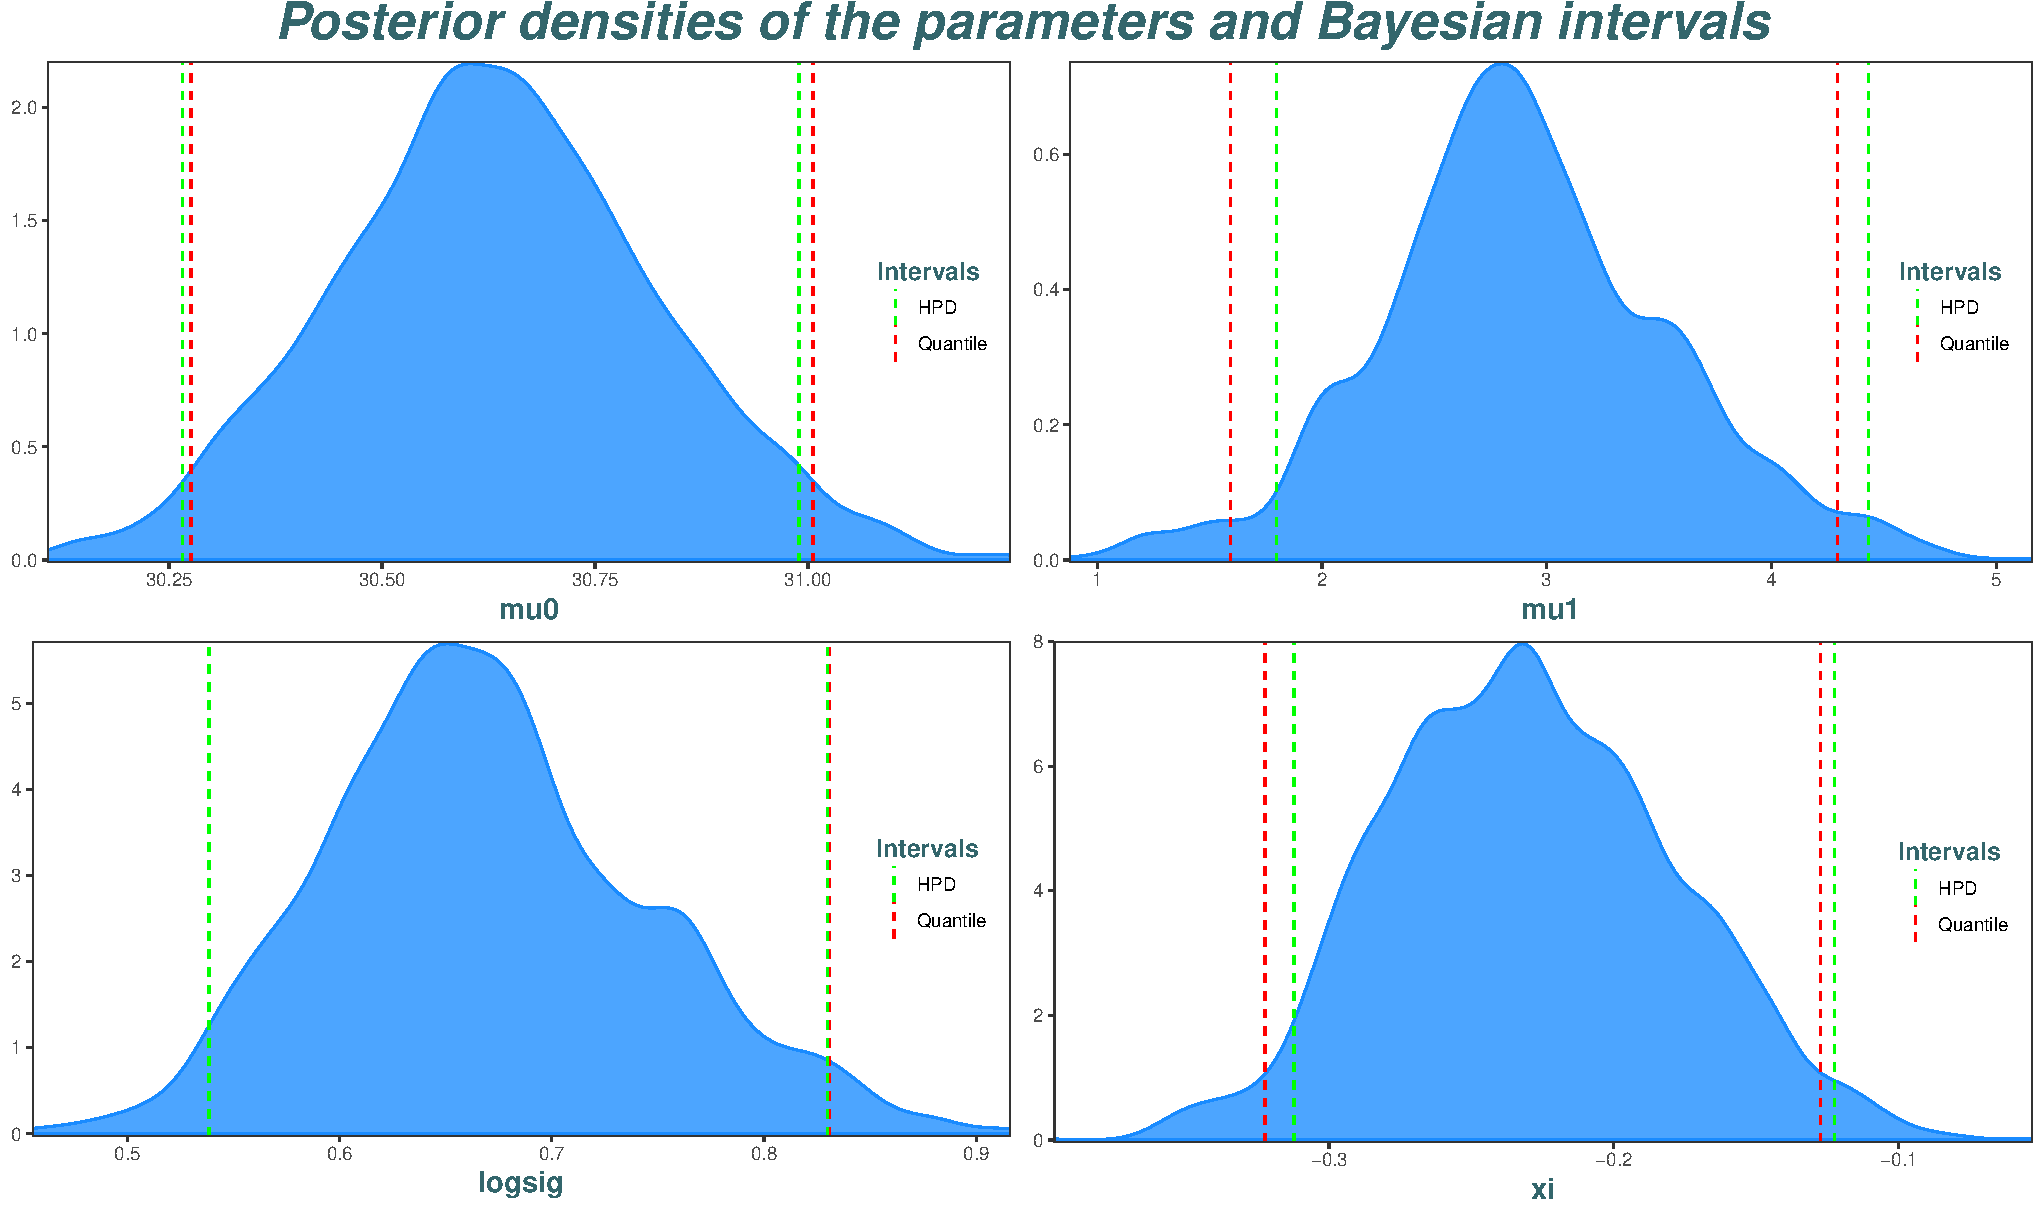
\includegraphics[width=0.8\linewidth]{postdens.pdf}\caption{Markov chains' Kernel posterior densities for the parameters with their corresponding Bayesian intervals. A Gaussian kernel with a bandwidth calculated by the \citet[pp.48, (3.31)]{silverman_1986} "rule of thumb" for each parameter has been used. Note that we did not make the back rescaling from $t^*$ to $t$ for this plot, which explains the values of $\mu_1$.}\label{fig:postdens}
\end{figure}
 We have added their corresponding $95\%$ Bayesian intervals (see \hyperref[bayes_cred_int]{Section \textbf{\ref{bayes_cred_int}}}. 
We can see the differences between the two intervals when the densities are not symmetric. In this case, the highest-posterior density (HPD) intervals are slightly more precise, and should be preferred.

This Figure \ref{fig:postdens} brings a great advantage of displaying the complete probability distributions of each parameters. We see here that all the probability mass for the shape parameter is below $0$, i.e. $\Pr \big\{\xi>0\big\}=0$, reinforcing our confidence that we are under an EV-Weibull model. %without any doubts.
Nevertheless, this should be tempered by caution since by relaunching the same model a high number of times, we obtained results where $\Pr \big\{\xi>0\big\}>0$, with a very small probability. This should lead us to consider sensitivity analysis.

These results are also summarized in Table \ref{tab:postq}.
\begin{table}[!htbp] \centering 
	\caption{Table of quantiles and \textbf{mean} of $\pi(\theta|\boldsymbol{x})$. Here, we transformed back $\mu_1$ from $t^*$ to $t$ in years for comparisons with frequentist results. } \label{tab:postq} 
	\begin{tabular}{@{\extracolsep{5pt}} c|cccccc} 
\toprule
		& 2.5\% & 25\% & 50\% &  \textbf{mean} & 75\% & 97.5\% \\ 
\midrule
		$\mu_0$  & $30.276$ & $30.511$ & $30.632$ & $30.633$ & $30.754$ & $31.006$ \\ 
		$\mu_1$ & $0.0136$ & $0.0214$ & $0.0245$ & $0.0248$ & $0.0282$ & $0.0367$ \\ 
		$\log\sigma$ & $0.539$ & $0.617$ & $0.663$ &  $0.669$ &$0.717$ & $0.831$ \\ 
		$\xi$ & $-0.323$ & $-0.266$ & $-0.232$ & $-0.230$ & $-0.195$ & $-0.127$ \\ 
\bottomrule
		\end{tabular} 
\end{table} 

Depending on the shape of the distribution, the median or the mean will generally be preferred as estimate. Comparing these results with the frequentist in Table \ref{tab:estliknsta} we can appreciate that these are very similar. The value of $\xi$, $\sigma$  and $\mu_0$ are slightly higher in the Bayesian results, but not significantly. Moreover, the most important parameter for our nonstationary analysis, $\mu_1$, has the same value at $3$ decimal places. We see from Figure \ref{fig:postdens} that it has a more peaked density distribution. Hence, the interpretation made with this model still holds. 

		
\subsection{Posterior Predictive Distribution} 

The Posterior Predictive Distribution (PPD) is a pure Bayesian method of inference that allows to make inference for predictions relying on the posterior results, as presented in \hyperref[sec:ppd]{Section \textbf{\ref{sec:ppd}}}. The primary objective is often prediction, in the sense that it is of interest to extrapolate the annual maxima in Uccle and for example predict the range of values that would take these maxima in order to have an idea, say, on the extreme heat waves that could occur in the future. 


To compute this PPD from (\ref{eq:ppd}), we expressly took a range of $116$ years in the future, as we know that it is not recommended to make very long-term extrapolations. We first depict the results in Figure \ref{fig:ppd} where we represent the PPD by its $95\%$ credible intervals, together with the observed values from $1901$ to $2016$ and the values from $2016$ to $2131$ that have been simulated from this PPD (\ref{eq:ppddd}).

 \begin{figure}[!htb]
 	\centering	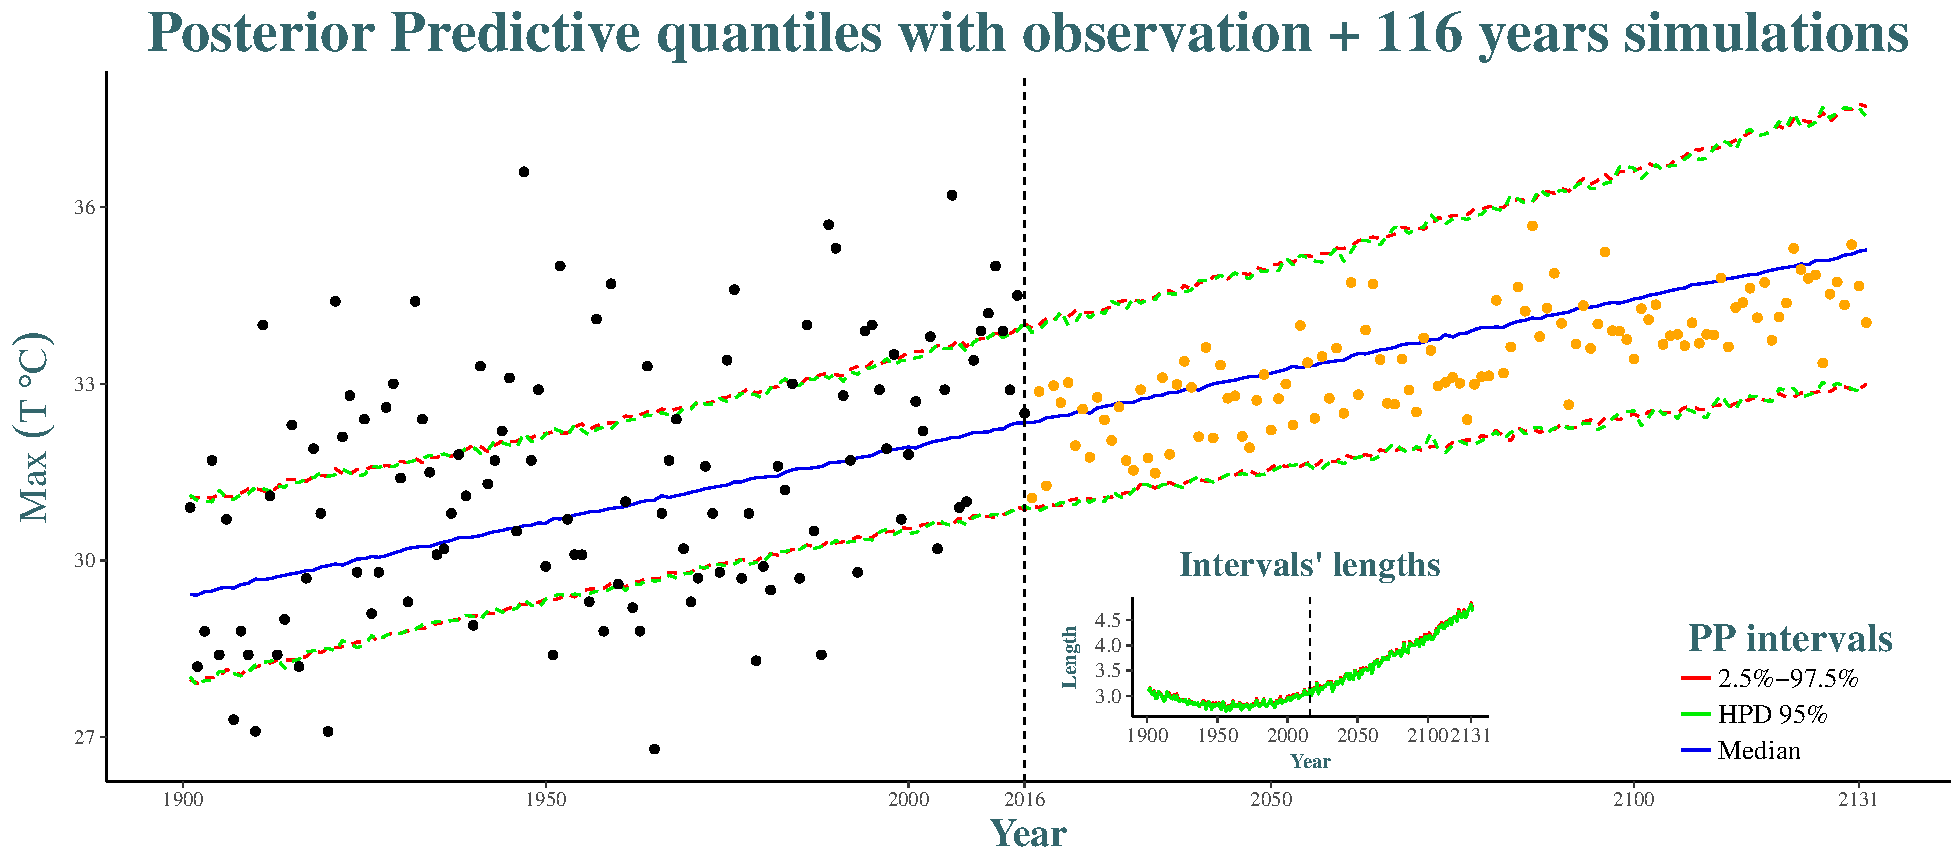
\includegraphics[width=0.9\linewidth]{ppd.pdf}\caption{Black dots represent the observations while orange dots represented the simulated values from the PPD. The printed plot aims to conveniently display the differences between the upper and the lower bounds of the two credible intervals considered.}\label{fig:ppd}
 \end{figure}
 
 We can clearly see on this Figure \ref{fig:ppd} the linear trend that is actually modeled by a linear model on the location parameter of the posterior distribution.  Indeed, we see from (\ref{eq:ppddd}) the contribution of the posterior to the PPD. 
 This Figure \ref{fig:ppd} also clearly highlights that the PP intervals are not $95\%$ credible intervals for the observed values but rather intervals for the posterior predicted values. Indeed, coverage analysis shows that the PP intervals cover $95\%$ of the simulated values from the PPD as the number of simulations becomes very high, but only $\approx 50\%$ for the observed values. The HPD and the quantile-based credible intervals are very similar here, for all the observations or simulations. 
  However, we can see that these intervals are taking the uncertainty of predicting in the future into account as they exponentially increase beyond the range of data. 
 In fact, the evolution of the PP quantiles is linear when in the range of data, and so is the PP median even beyond the range of the data. But, when extrapolation begins, the PP upper quantiles will have an increasing slope over time while the PP lower quantiles will have a decreasing slope.
 
 To better understand the PPD with a global view and in order to obtain a more convenient visual quantification of the predictive uncertainty over time, we present Figure \ref{fig:post_pred}.

 \begin{figure}[!htb]
  	\centering	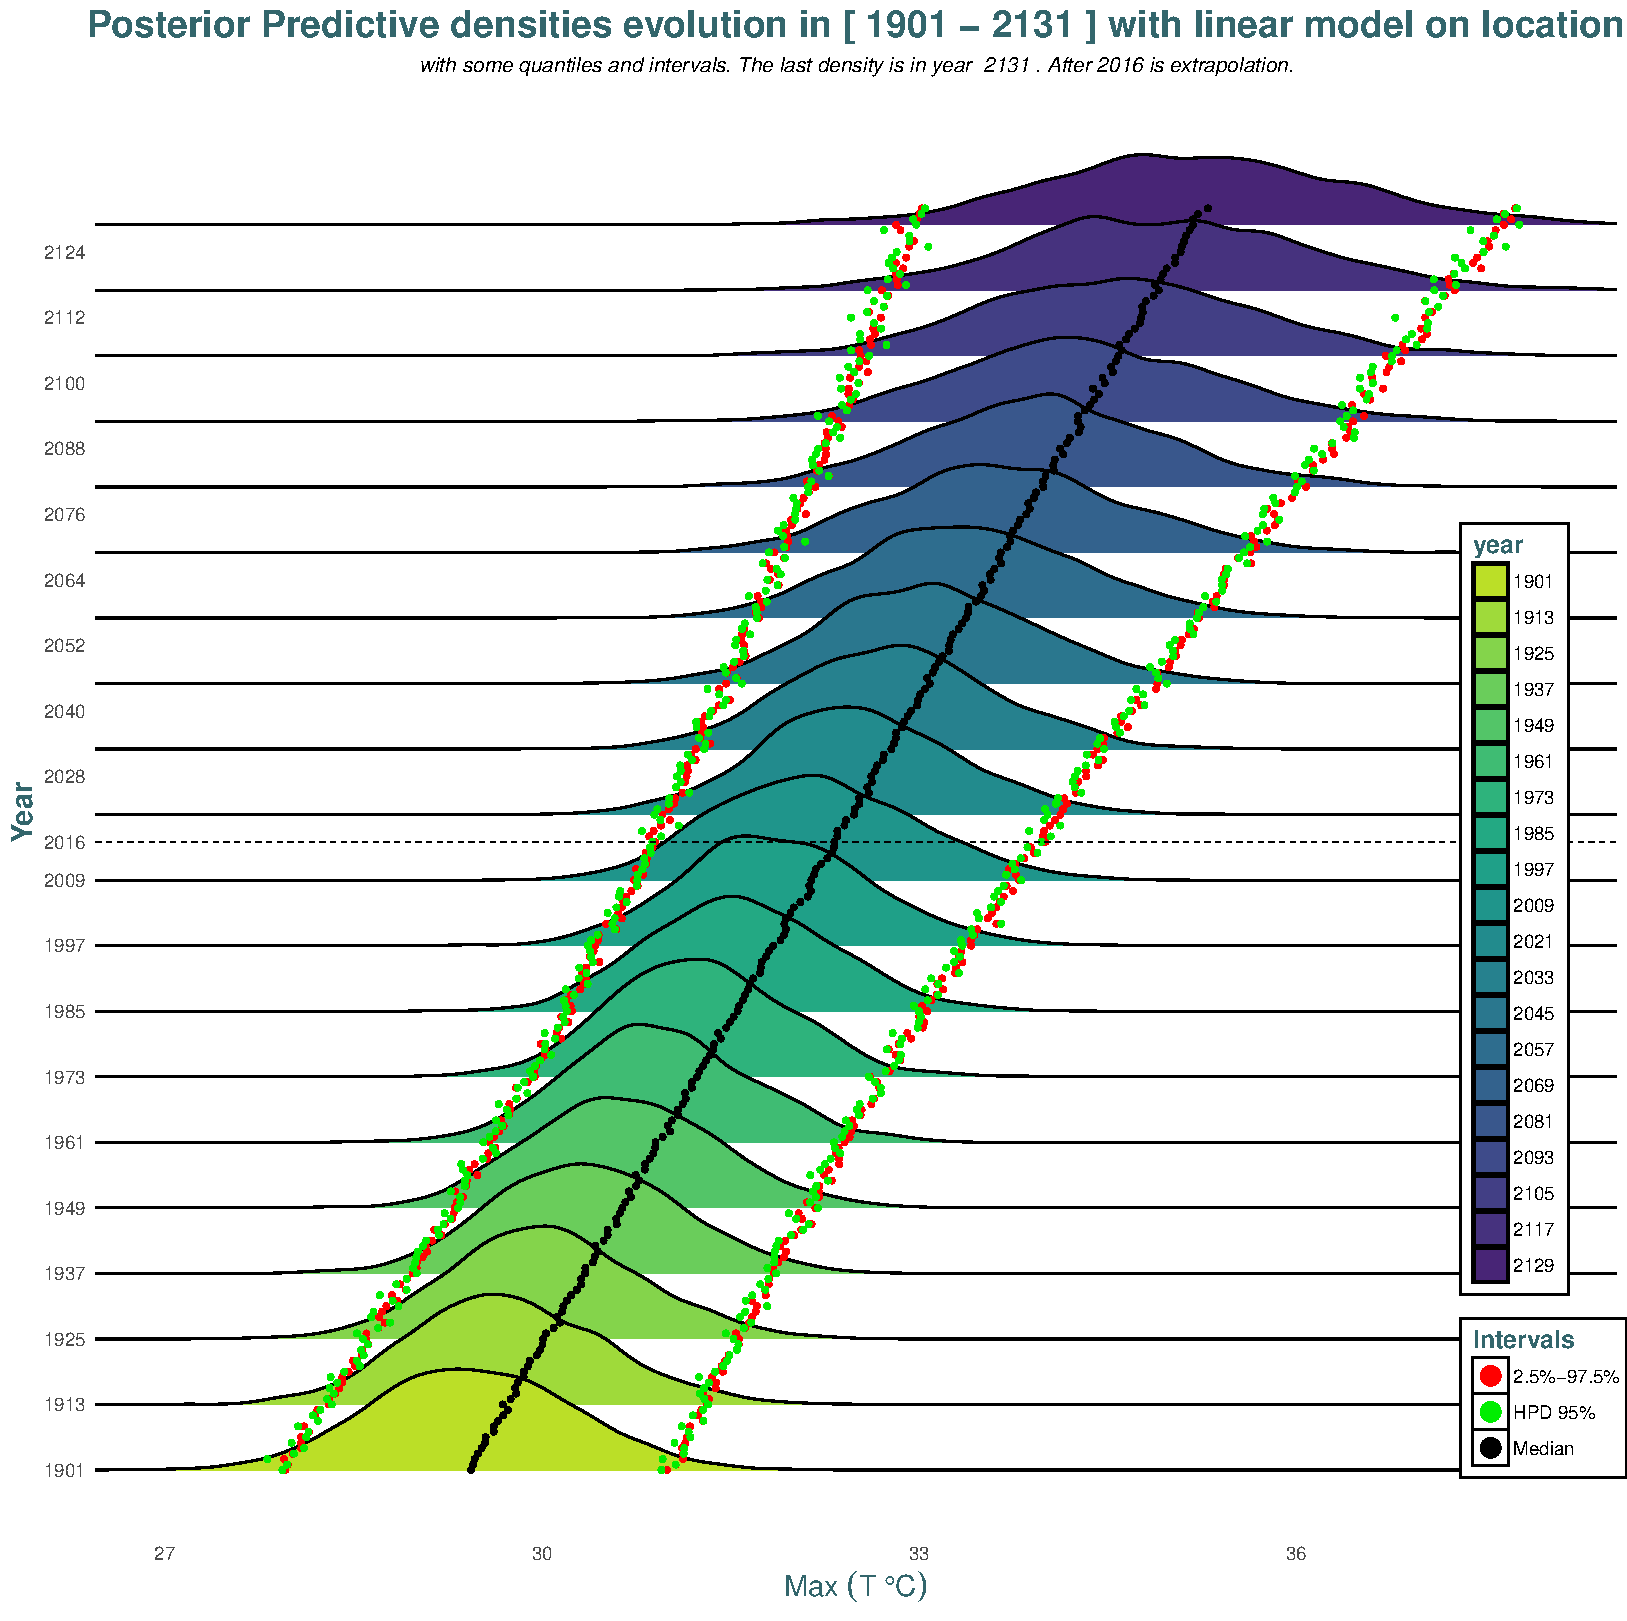
\includegraphics[width=0.8\linewidth]{predpred.pdf}\caption{Visualization of the PPD from $1901$ and extrapolated to year $2131$. $20$ densities are drawn in this range by steps of $12$ years. Quantiles are displayed for every years.  A Gaussian kernel with a joint bandwidth calculated by the \citet[pp.48, (3.31)]{silverman_1986} "rule of thumb" is picked for each densities.}\label{fig:post_pred}
 \end{figure}
  
  From this Figure \ref{fig:post_pred},  we also notice the linear trend and we visualize more clearly the evolution of the quantiles over time with their gap increasing after $2016$, i.e. their deviation from the median. This comes from the density distributions that become more and more flat after $2016$, indicating an increasing variance and hence the inclusion of the prediction uncertainty. 

Interesting informations can come from these PP plots when considering other models, and the shape of the predictive densities is sometimes. But, the parametric models from Table \ref{tabe:comp_mod_bay} are rather limited, and other models could be developed. For example, step-change models, or to obtain flexible models by following the idea of \hyperref[sec:nnxp]{Section \textbf{\ref{sec:nnxp}}}, it would be very interesting to consider \emph{Bayesian Neural Networks}.

\subsection{Return Levels}


We remind that quantiles of the fitted distribution can be more conveniently interpreted in EVT as returns levels. 
 Here, for the quantiles depicted above it is different since we are under the fitted PP distribution and not the fitted distribution. Indeed, these quantiles are taking the uncertainty of future prediction into account and are thus not strictly linearly increasing. In fact, considering quantiles in extreme tails will increasingly raise the gap between these quantiles, as the PPD will become increasingly flat and will allow for increasingly more extreme values. Yet, we have seen in Figure \ref{fig:rl_nsta} that the increase of the return levels was strictly linear even beyond the range of the data, although it was the same nonstationary model in a frequentist setting.
 
In fact, the quantiles of the PPD depicted in Figure \ref{fig:ppd} or \ref{fig:post_pred} are commonly called \emph{predictive return levels}. For example the above red line in Figure \ref{fig:ppd} is actually the $40$-year predictive return levels.

It is still also possible to compute the returns levels as in Figure \ref{fig:rl_nsta} by simply estimating the parameters (e.g. by their MC's posterior mean or median from Table \ref{tab:postq}). Then, the GEV model will be fit and the corresponding return levels can be computed from this nonstationary GEV model. Relying on the median, we verified that the return levels line is nearly the same for all points since the parameter's values are very close ; Bayesian return levels having a slightly higher intercept and slightly smaller slope compared to the blue line in Figure \ref{fig:rl_nsta}. 


\section{Remarks and Comparison with Frequentist results}\label{sec:rem}


In this analysis, we relied on Bayesian inference to complement the nonstationary analysis started in \hyperref[sec:anagev]{sec:anagev}. 
As we noticed, comparing Table \ref{tab:postq} with Table \ref{tab:estliknsta} yielded very similar results. This is natural and this is rather comforting as we used non-informative priors so far.

As this is the last section, we wanted to gather all the results we've had during this thesis in one graph that could summarize the information in the most efficient way.
The following Figure \ref{fig:cicomp} compares several parameters' confidence intervals that have been computed during this thesis. 

\begin{itemize}
	\item The \emph{frequentist} confidence intervals computed in
	\hyperref[sec:xpstatio]{Section \textbf{\ref{sec:xpstatio}}}, comprising those coming from the normal approximation of the MLE and the profiled likelihood intervals.
	\item The \emph{bootstrap} confidence intervals computed in  \hyperref[sec:boot]{Section \textbf{\ref{sec:boot}}} for the nonstationary model with  a linear model on the location only. We show the residual but also the parametric bootstrap method. These intervals have not been computed for the location parameters since these were directly computed for $\mu(t)$ rather than $\mu_0$ and $\mu_1$. From the particular nature of these intervals which estimate parameters by GML and make use of prior distribution to compute the GEV-CDN weights, we will not consider these as truly "frequentist", but this is debatable.
	\item The \emph{Bayesian} credible intervals seen and discussed above in \hyperref[sec:bayinfci]{Section \textbf{\ref{sec:bayinfci}}}.
\end{itemize}

\begin{figure}[!htb]
	\centering	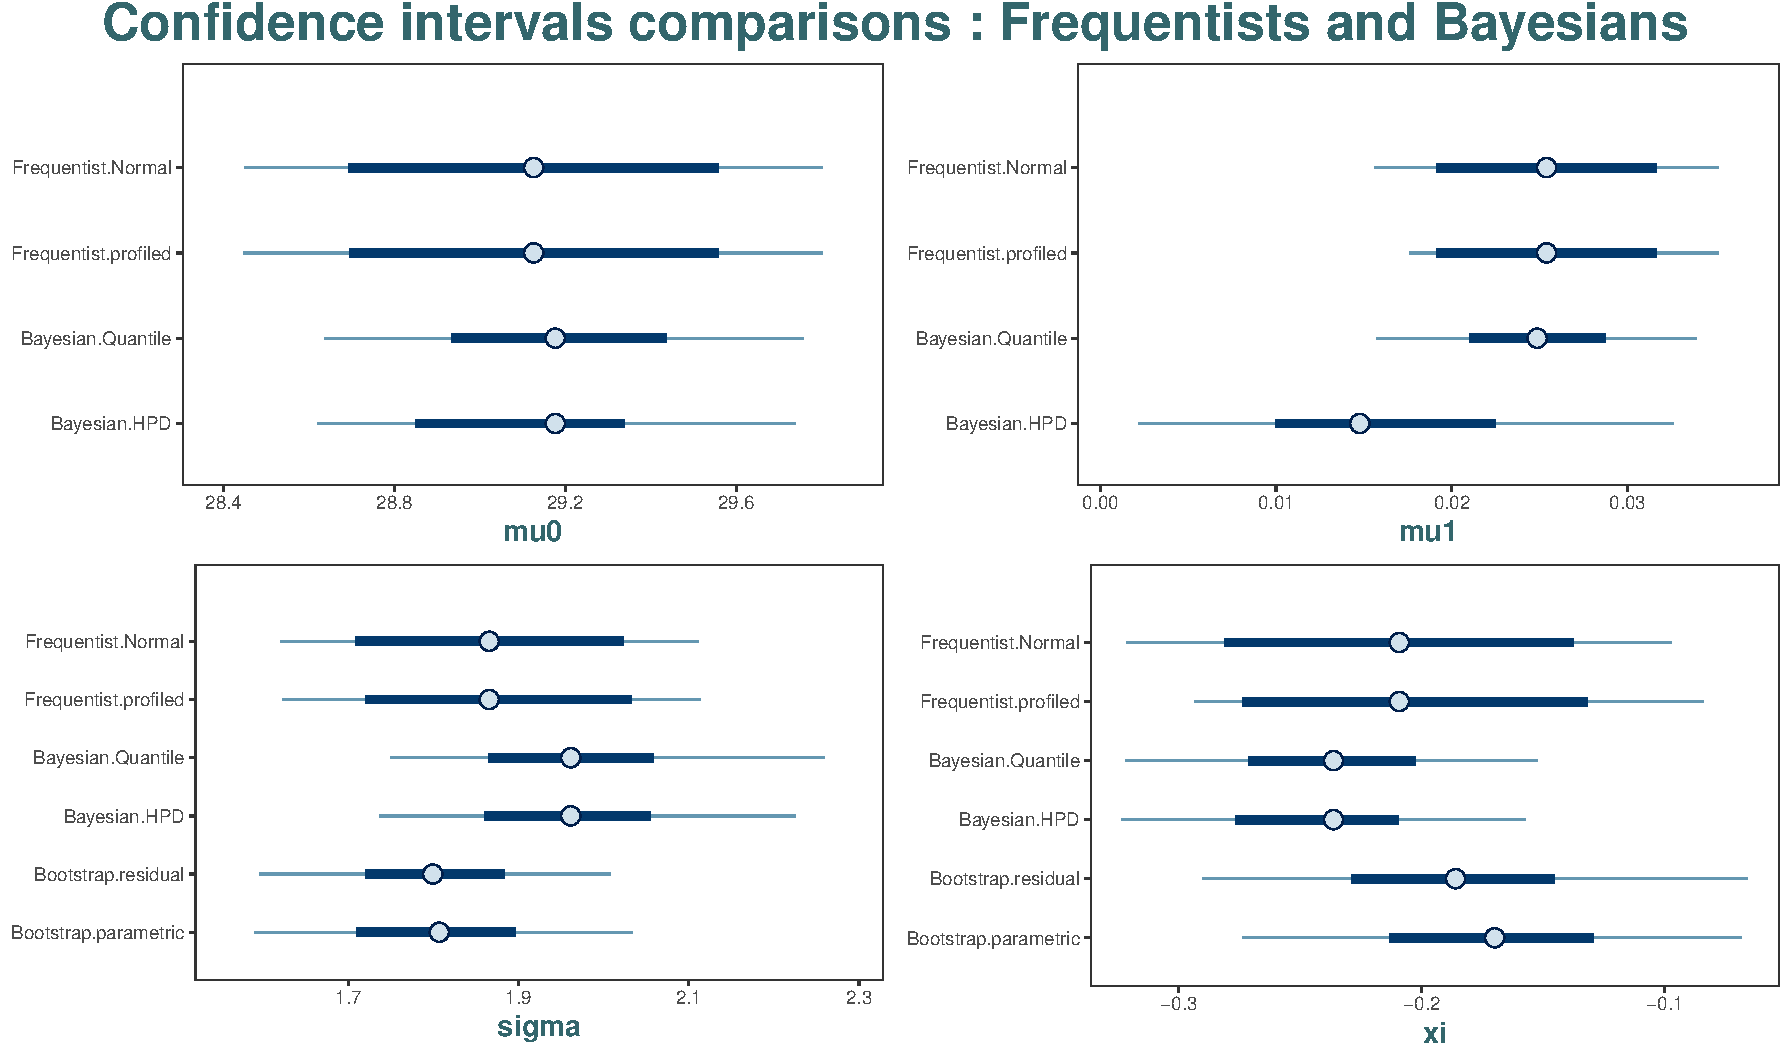
\includegraphics[width=0.9\linewidth]{cicomp.pdf}\caption{The center of the interval is the MLE for the frequentist intervals and the posterior median for the Bayesian intervals. Thicker lines indicate $50\%$ confidence (or credibility) intervals while thinner lines indicate $95\%$ intervals.}\label{fig:cicomp}
\end{figure}

By using objective priors (i.e. priors with very large variance), we should obtain the same results in the frequentist and in the Bayesian setting, which will be a prove of robustness of these results. However, the way of computing the intervals are intrinsically different and hence, the observed differences between these intervals is a rather a difference of point of view.

Note that the large differences between the Bayesian and the frequentist intervals for the parameter $\mu_0$ are probably due to the difficulties faced by the rescaling of the parameter $\mu_1$ and has influence on the distribution of $\mu_0$. The same argument goes for the Bayesian HPD for $\mu_1$ where the reparametrization with $t$ brought problems.


\subsubsection*{Discussion on the Prior : Sensitivity Analysis}

In all the provided analysis, we were not able to introduce knowledge through the specification of the prior. Hence, we have used non-informative priors (see \hyperref[sec:noninfoprior]{Section \textbf{\ref{sec:noninfoprior}}}), and in particular \emph{vague} (near-flat) independent normally distributed \emph{priors} (\ref{eq:vagprior}) for each parameter since this is the most convenient way to express our ignorance.
%\textbf{section 7.4} evdbayes pdf + suppplément risk book 

The basic method of sensitivity analysis is to fit several models to the same problem. From our prior ignorance, it was not relevant to analyze the sensitivity from the prior. 
Even if the considered nonstationary models were limited here, it could be the case that several models provide an adequate fit to the data. In this case, sensitivity analysis could determine by what extent posterior inferences change when alternative models are used.
This includes posterior distributions of the parameters but also PPD. This would interesting to consider if we have adequate models, but when looking at Table \ref{tab:comp_mod_bay}, it is rather hazardous. 
Note that the sensitivity of the marginal posterior density of the shape parameter $\xi$ is often of particular interest


\subsubsection*{Bayesian Model Averaging}\label{sec:bmaxp}

Since we were not able to strictly select one model in a Bayesian fashion with the Bayes factor in \hyperref[sec:baycomp]{Section \textbf{\ref{sec:baycomp}}}, Bayesian Model Averaging could an idea to prevent us from fitting one single model that could be wrong.
This idea that follows the one of the ensemble model such as bagging used in \hyperref[sec:xpbagg]{Section \textbf{\ref{sec:xpbagg}}}. However, this method is beneficial either when we have a large amount of models that could prepresent a great part of the process, or when the models at hand are really informative for the process, which is not the case here.



